\documentclass[12pt, a4paper]{article}
\usepackage[bottom=2cm,top=3cm,left=3cm,right=2cm]{geometry}
\usepackage[brazilian]{babel} % Traduz alguns termos para o português
\usepackage[utf8]{inputenc} % Reconhece acentuação
\usepackage{color,graphicx}
\usepackage{enumerate}
\usepackage{mathtools}
\usepackage{listings}
\usepackage{hyperref}
\hypersetup{
	colorlinks=true,     
	urlcolor=blue
}

\definecolor{olive}{RGB}{175,128,0}
\definecolor{Aquamarine}{RGB}{0,175,175}

\usepackage{setspace}
\onehalfspacing	
\setlength{\parindent}{30pt}

\usepackage{indentfirst}

\title{
	\begin{large}
		Laboratório 1: Computação Evolucionária - 2016/2
	\end{large}}
\author{Alunos: Davi Viana e Rafael Castro}
\date{30/08/2016}

\begin{document}
	\maketitle
	
	\vspace*{-7.5cm}
	{\bf
		\begin{center}
			{\large
				\hspace*{0cm}Universidade Federal de Minas Gerais} \\
			\hspace*{0cm}Engenharia de Sistemas  \\
		\end{center}
	}
	\vspace*{5cm}
	
\section{Gráficos das Execuções do Algoritmo Genético}
\par Seguem os gráficos das execuções do algoritmo genético para N=8, N=20 e N=50, sendo que o tamanho da população para todos os casos é 50. Em todos os gráficos, o eixo das abscissas indica a geração e o eixo das ordenadas indica a qualidade da solução: em verde é possível ver as médias das populações e em azul o melhor valor.
\begin{figure}[h]
	\centering
	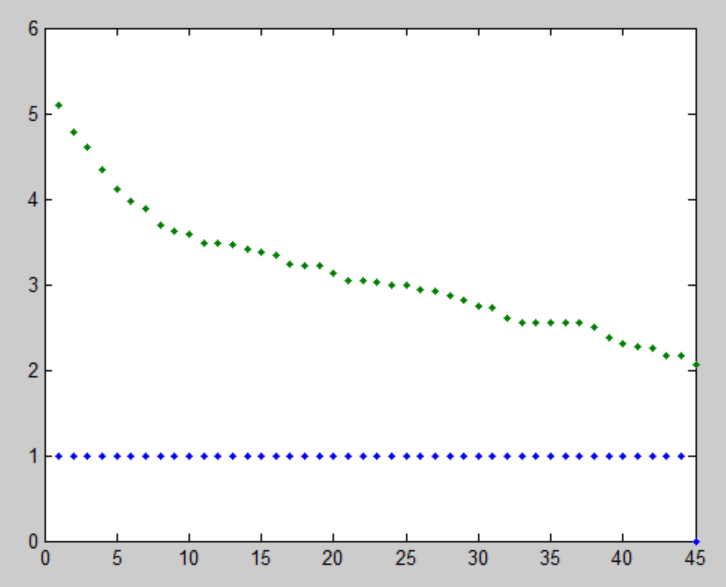
\includegraphics[width=15cm]{img/n8.png}
	\caption{N igual a 8 e Tamanho da população igual a 50}
	\label{fig:n8}
\end{figure}  

\begin{figure}[h]
	\centering
	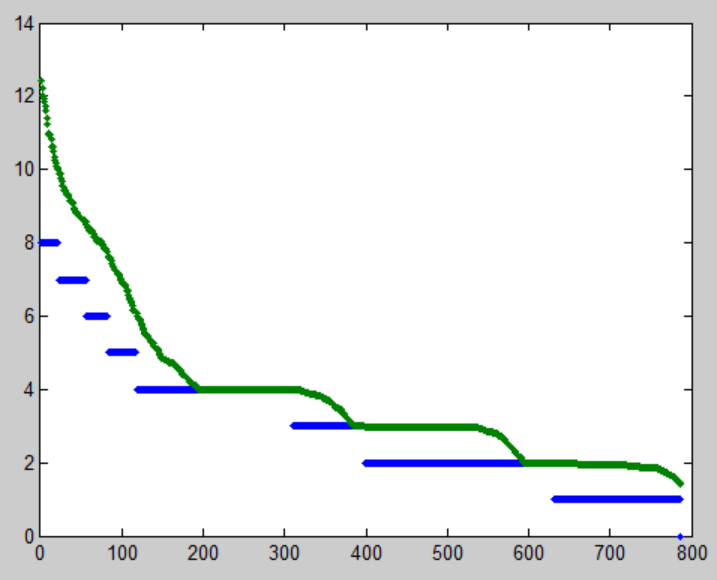
\includegraphics[width=15cm]{img/n20.png}
	\caption{N igual a 20 e Tamanho da população igual a 50}
	\label{fig:n20}
\end{figure}  

\begin{figure}[h]
	\centering
	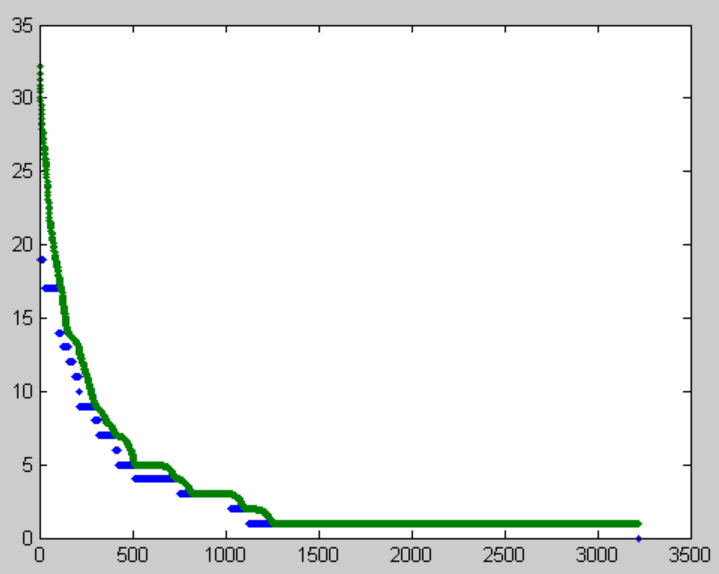
\includegraphics[width=15cm]{img/n50.png}
	\caption{N igual a 50 e Tamanho da população igual a 50}
	\label{fig:n50}
\end{figure}  
		
\end{document}